\subsection{Классификация коммутативных колец}

На данный момент мы получили следующую классификацию коммутативных колец:
\begin{center}\begin{tikzcd}[row sep = tiny, column sep = small, font = \footnotesize]
	&&\stackanchor{Факториальные}{кольца}\arrow[phantom, sloped, yshift=2pt, xshift=2pt]{dr}{\supset}&&&\\
	\stackanchor{Коммутативные}{кольца} \arrow[phantom]{r}{\supset} &\stackanchor{Области}{целостности}\arrow[phantom, sloped, yshift=-2pt]{ur}{\supset}\arrow[phantom, sloped, yshift=2pt, xshift=-2pt]{dr}{\supset}&&\stackunder{\stackon{главных}{Кольца}}{идеалов}\arrow[phantom]{r}{\supset}&\stackanchor{Евклидовы}{кольца}\arrow[phantom]{r}{\supset}&{\text{Поля}}\\
	&&\stackanchor{Нетеровы}{кольца}\arrow[phantom, sloped, yshift=-2pt, xshift=2pt]{ur}{\supset}&&&
\end{tikzcd}\end{center}

Более того, для большей части вложений мы можем привести контрпримеры, показывающие, что эти вложения являются строгими:
\begin{itemize}
	\item $\Z_n$ при составных $n \in \N$ "--- коммутативное кольцо, но не область целостности
	\item $\Z[2i]$ "--- область целостности и даже нетерово кольцо, но не факториальное кольцо
	\item $\Q[x_1, x_2, \dotsc]$ "--- область целостности и даже факториальное кольцо, но не нетерово кольцо
	\item $\Z[x]$ "--- факториальное и нетерово кольцо, но не кольцо главных идеалов
	\item $\Z$ "--- евклидово кольцо, но не поле
\end{itemize}

Остается привести контрпример кольца главных идеалов, не являющегося евклидовым. Для этого до конца раздела зафиксируем кольцо $\Z[\alpha]$, где $\alpha := \frac{-1 + \sqrt{19}i}2$ "--- корень многочлена $x^2 + x + 5$.

\begin{theorem}
	Кольцо $\Z[\alpha]$ не является евклидовым.
\end{theorem}

\begin{proof}
	Рассмотрим стандартную для комплексных чисел норму: $\forall a + b\alpha \hm\in \Z[\alpha]: N(a + b\alpha) \hm= a^2 - ab + 5b^2$. Легко видеть, что только только числа $\pm1$ в $\Z[\alpha]$ имеют норму, равную единице, поэтому $\Z[\alpha]^* = \{\pm1\}$.
		
	Предположим, что $\Z[\alpha]$ "--- евклидово кольцо с нормой $\overline{N}$. Пусть $x \in \Z[\alpha]$ "--- необратимый элемент с наименьшей нормой. Так как $\forall y \in \Z[\alpha]$, $y \mid x: \overline{N}(y) < \overline{N}(x)$ или $y \in \Z[\alpha]^*$, то $x$ неразложим. По предположению, $\Z[\alpha]$ является, в частности, кольцом главных идеалов, поэтому элемент $x$ прост и $\Z[\alpha] / (x)$ "--- поле.
	
	Поскольку $x$ необратим, то $|\Z[\alpha] / (x)| > 1$. Норма элемента $x$ минимальна, поэтому при делении на $x$ в $\Z[\alpha]$ остатками могут быть только числа $0$ и $\pm1$. Значит, либо $\Z[\alpha] / (x) \cong \Z_2$, либо $\Z[\alpha] / (x) \cong \Z_3$. Рассмотрим образ числа $\alpha$ при действии канонического эпиморфизма $\pi: \Z[\alpha] \to \Z[\alpha] / (x)$. Поскольку $\alpha^2 + \alpha + 5 = 0$, то либо $\pi(\alpha)^2 + \pi(\alpha) + 1 \equiv_2 0$, либо $\pi(\alpha)^2 + \pi(\alpha) + 2 \equiv_3 0$. Но ни одно из этих сравнений не может быть выполнено. Значит, кольцо $\Z[\alpha]$ "--- не евклидово.
\end{proof}

\begin{proposition}
	Пусть $K$ "--- область целостности. Тогда $K$ является кольцом главных идеалов $\lra$ определена функция $N: K\backslash\{0\} \to \N \cup \{0\}$ такая, что $\forall a, b \in K\backslash\{0\}: b \mid a$ или $\exists q, s \in K: N(as - bq) < N(b)$.
\end{proposition}

\begin{proof}~
	\begin{itemize}
		\item[$\ra$] Пусть $K$ "--- кольцо главных идеалов и $a, b \in K\backslash\{0\}$. Если $b \nmid a$, то $(a, b) = (d)$ для некоторого $d \in K\backslash\{0\}$, причем $d$ "--- наибольший общий делитель $a, b$. Значит, если в качестве <<нормы>> $N$ взять число неразложимых элементов в разложении данного элемента, то $\exists q, s \in K: d = as - bq \ra N(as - bq) < N(b)$.
		\item[$\la$] Легко проверить, что если $I$ "--- ненулевой идеал в $K$, то элемент $d \in I \backslash \{0\}$ с минимальной <<нормой>> $N$ порождает $I$.\qedhere
	\end{itemize}
\end{proof}

\begin{theorem}
	$\Z[\alpha]$ является кольцом главных идеалов.
\end{theorem}

\begin{proof}
	Рассмотрим стандартную комплексную норму $N$ на $\Z[\alpha]$ и произвольные $a, b \in \Z[\alpha] \backslash \{0\}$ такие, что $b \nmid a$. Проверим, что $\exists q, s \in \Z[\alpha]: N(as - bq) < N(b)$, то \pagebreak есть $N(\frac {sa}b - q) < 1$. Если число $\frac ab$ попадает в одну из полос радиуса $\frac{\sqrt{3}}2$, построенных на прямых $\im{z} = \im\alpha k$, $k \in \Z$, то можно подобрать такое $q \in \Z[\alpha]$, что $N(\frac ab - q) < 1$. Если же число $\frac ax$ не попадает ни в одну из полос, то легко убедиться, что тогда в одну из полос попадает число $\frac {2a}b$. Данное рассуждение проиллюстрировано ниже:
	\begin{center}
		\scalebox{0.85}{
			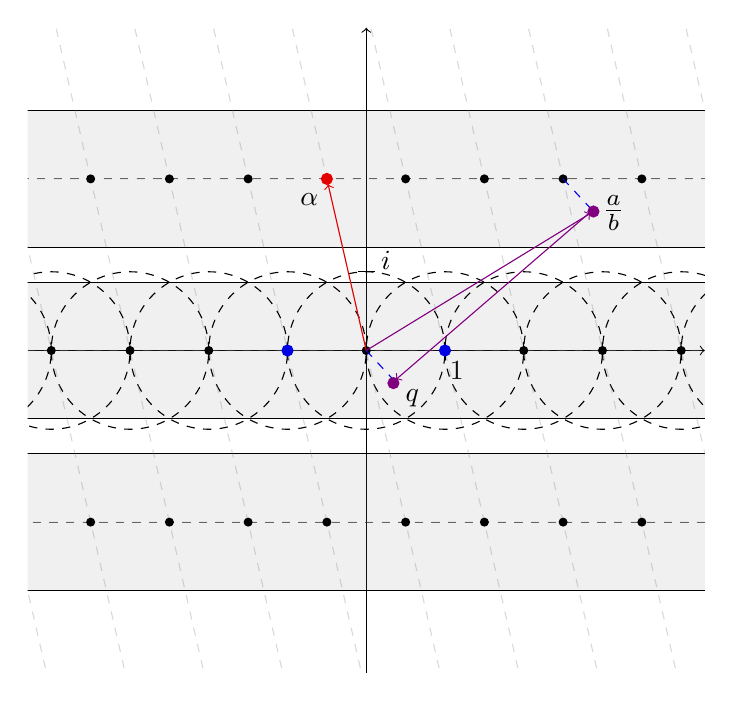
\begin{tikzpicture}
				\clip (-4.3, -4.1) rectangle (4.3, 4.1);
				\draw [->] (-4.3, 0) -- (4.3, 0);
				\draw [->] (0, -4.1) -- (0, 4.1);
				
				\draw (1,3pt) -- (1,-3pt);
				\draw (3pt,1) -- (-3pt,1);
				
				\node at (1.15, -0.25) {$1$};
				\node at (0.25, 1.15) {$i$};
				
				\filldraw[fill=gray, fill opacity=0.12, draw=black] (-6,4.35889894/2 + 1.7320501/2) rectangle (6,4.35889894/2-1.7320501/2);
				\filldraw[fill=gray, fill opacity=0.12, draw=black] (-6,1.7320501/2) rectangle (6,-1.7320501/2);
				\filldraw[fill=gray, fill opacity=0.12, draw=black] (-6,-4.35889894/2 + 1.7320501/2) rectangle (6,-4.35889894/2-1.7320501/2);
				
				\foreach \x in {-6, -5, ..., 6}{
					\draw[black, dashed] (\x, 0) circle[radius=1];
				}
				
				\pgftransformcm{1}{0}{-1/2}{4.35889894/2}{\pgfpoint{0cm}{0cm}}
				\draw [dashed, opacity=0.6] (-6, 1) -- (6, 1);
				\draw [dashed, opacity=0.6] (-6, -1) -- (6, -1);
				\draw[style=help lines,dashed, thin, gray, opacity=0.3] (-6,-6) grid (6,6);
				
				\foreach \x in {-6, -5, ..., 6}{
					\foreach \y in {-6, -5, ..., 6}{
						\node[draw,circle,inner sep=1pt,fill] at (\x, \y) {};
					}
				}
				\node[draw,circle,inner sep=1.4pt,fill,black!10!blue] at (-1, 0) {};
				\node[draw,circle,inner sep=1.4pt,fill,black!10!blue] at (1, 0) {};
				\node[draw,circle,inner sep=1.4pt,fill,black!10!red] at (0, 1) {};
		
				\draw [->, black!10!red] (0, 0) -- (0, 0.97) node [black, below left] {$\alpha$};
				
				\draw [dashed, black!10!blue] (3, 1) -- (3.29, 0.81) {};
				\draw [dashed, black!10!blue] (0, 0) -- (0.29, -0.19) {};
				\draw [->, violet] (0, 0) -- (3.25, 0.8) node [black, right, scale = 1.2] {$\frac ab$};
				\node[draw,circle,inner sep=1.4pt,fill,violet] at (3.29, 0.81) {};
				\draw [->, violet] (3.29, 0.82) -- (0.29, -0.17) node [black, below right] {$q$};
				\node[draw,circle,inner sep=1.4pt,fill,violet] at (0.25, -0.19) {};
			\end{tikzpicture}
		}
	\end{center}
	
	Таким образом, стандартная комплексная норма на $\Z[\alpha]$ удовлетворяет условию, что $\forall a, b \in \Z[\alpha]\backslash\{0\}: b \mid a$ или $\exists q, s \in \Z[\alpha]: N(as - bq) < N(b)$. Значит, $\Z[\alpha]$ "--- кольцо главных идеалов.
\end{proof}